\documentclass[aspectratio=169,
hyperref={colorlinks,urlcolor=blue}
]{beamer}


%\usetheme{Pittsburgh}
\usetheme{default}
\usepackage{colortbl}%colored tables
%For using helvetica font:
\usepackage[scaled]{helvet}
\usepackage[T1]{fontenc}
\renewcommand\familydefault{\sfdefault}
\urlstyle{same} %sets the fonts for urls
\usepackage{pdfpages}
\usepackage{siunitx}
\usepackage{caption}
\usepackage{pifont}%for dings
\usepackage{pgfplots}%for 3d plotting
\pgfplotsset{compat = newest}
\usepackage{mathtools}%box in align env \Aboxed
\usepackage[american,smartlabels]{circuitikz}%for drawing circuits
\usepackage{multimedia}
\usepackage{animate}
\usepackage{xcolor}


\usetikzlibrary{arrows}
\usetikzlibrary {3d} 
\usetikzlibrary{decorations.markings, math}
\usetikzlibrary{intersections, pgfplots.fillbetween}
\usetikzlibrary {shapes.geometric} 


%\definecolor{myblue}{RGB}{5, 34, 150}
\definecolor{myblue2}{RGB}{5, 34, 150}
\definecolor{myblue}{RGB}{0,36,82}
\definecolor{myred}{RGB}{207, 2, 13}
\definecolor{mygreen}{RGB}{0, 158, 11}
\definecolor{myyellow}{RGB}{220,220,0}
\definecolor{qblue}{RGB}{0,36,82}
\definecolor{qgold}{RGB}{250,189,15}
\definecolor{qred}{RGB}{185,14,49}
\definecolor{cblue}{rgb}{0.13, 0.67, 0.8}
\definecolor{corange}{rgb}{0.8, 0.34, 0.0}
\definecolor{cpurple}{rgb}{0.54, 0.29, 0.42}

%%%%%%%%%%%% General settings
\setbeamercolor{frametitle}{fg=black}
\setbeamercolor{title}{fg=black}
\setbeamercolor{author}{fg=myblue2}

\beamertemplatenavigationsymbolsempty %no navigation controls at bottom of slides
%\setbeamertemplate{footline}[frame number]
\usefonttheme{professionalfonts} 
\setbeamerfont{title}{series=\bfseries,parent=structure}
\setbeamerfont{frametitle}{series=\bfseries,parent=structure}

%%%%%%%%%%%%Lists
\setbeamertemplate{itemize item}[circle] %{\color{myblue}$\circ$}
\setbeamertemplate{itemize subitem}{\color{myblue2}$\circ$}
\setbeamertemplate{itemize subsubitem}{\color{myblue2}$\cdot$}
\setbeamercolor{itemize item}{bg=myblue2,fg=myblue2}
\setbeamercolor{enumerate item}{bg=myblue2,fg=myblue2}
%%%%%%%%%%%%%%%%%%%%%%%%%%%%

%%%%%%%%%%%%Blocks
\setbeamertemplate{blocks}[rounded]
%Default block
\setbeamercolor{block title}{bg=myblue2, fg=white}
\setbeamercolor{block body}{bg=myblue2!10}
\setbeamerfont{block body}{size=\scriptsize}
\setbeamerfont{block title}{size=\scriptsize}
%Alert block
\setbeamercolor{block title alerted}{bg= myblue2, fg=white}
\setbeamercolor{block body alerted}{bg=myblue2!10}
\setbeamerfont{block body alerted}{size=\scriptsize}
\setbeamerfont{block title alerted}{size=\scriptsize}
%example block
\setbeamercolor{block title example}{bg=mygreen, fg=white}
\setbeamercolor{block body example}{bg=mygreen!10}
\setbeamerfont{block body example}{size=\scriptsize}
\setbeamerfont{block title example}{size=\scriptsize}
%%%%%%%%%%%%%%%%55


%%%%%%%%%%%%Figures and captions
\captionsetup{font=scriptsize,labelfont=scriptsize}
%\setbeamertemplate{caption}{\raggedright\insertcaption\par}
\newenvironment{capfig}[3]{\begin{figure}\includegraphics[width=#1\textwidth]{#2}\caption*{\textit{#3}}\end{figure}}{}

%\makeatother
%\setbeamertemplate{footline}
%{
%  \leavevmode%
%  \hbox{%
%  \begin{beamercolorbox}[wd=.4\paperwidth,ht=2.25ex,dp=1ex,center]{author in head/foot}%
%    \usebeamerfont{author in head/foot}\insertshortauthor
%  \end{beamercolorbox}%
%  \begin{beamercolorbox}[wd=.6\paperwidth,ht=2.25ex,dp=1ex,center]{title in head/foot}%
%    \usebeamerfont{title in head/foot}\insertshorttitle\hspace*{3em}
%    \insertframenumber{} / \inserttotalframenumber\hspace*{1ex}
%  \end{beamercolorbox}
%  }%
%  \vskip0pt%
%}
%\makeatletter

\makeatother
\setbeamertemplate{footline}
{
  \leavevmode%
  \hbox{%
\begin{beamercolorbox}[wd=.27\paperwidth,ht=2.25ex,dp=1ex,center]{author in head/foot}%
    \color{black}{\insertinstitute}
\end{beamercolorbox}
  \begin{beamercolorbox}[wd=.27\paperwidth,ht=2.25ex,dp=1ex,center]{author in head/foot}%
    \color{black}{\inserttitle}
  \end{beamercolorbox}%
  \begin{beamercolorbox}[wd=.27\paperwidth,ht=2.25ex,dp=1ex,center]{title in head/foot}%
    \color{black}{\insertshortauthor}
  \end{beamercolorbox}
  \begin{beamercolorbox}[wd=.27\paperwidth,ht=2.25ex,dp=1ex,center]{title in head/foot}%
    \hspace{.28\paperwidth}\color{black} \insertframenumber{} / \inserttotalframenumber\hspace*{1ex}
  \end{beamercolorbox}
  }%
  \vskip0pt%
}
\makeatletter

\setbeamertemplate{title page}
{
  \begin{tikzpicture}[remember picture,overlay]
    \def\barh{4}%15
  
    \draw[color=myblue2,line width=\barh] ([yshift=-0.5*\barh]current page.north west) -- ([yshift=-0.5*\barh,xshift=-0.67\paperwidth]current page.north east);
    \draw[color=myblue2,line width=\barh] ([yshift=-0.5*\barh,xshift=-0.67\paperwidth]current page.north east) -- ([yshift=-0.5*\barh,xshift=-0.34\paperwidth]current page.north east);
    \draw[color=myblue2,line width=\barh] ([yshift=-0.5*\barh,xshift=-0.34\paperwidth]current page.north east) -- ([yshift=-0.5*\barh]current page.north east); 
  
    \draw[color=myblue2,line width=\barh] ([yshift=0.5*\barh]current page.south west) -- ([yshift=0.5*\barh,xshift=-0.67\paperwidth]current page.south east);
    \draw[color=myblue2,line width=\barh] ([yshift=0.5*\barh,xshift=-0.67\paperwidth]current page.south east) -- ([yshift=0.5*\barh,xshift=-0.34\paperwidth]current page.south east);
    \draw[color=myblue2,line width=\barh] ([yshift=0.5*\barh,xshift=-0.34\paperwidth]current page.south east) -- ([yshift=0.5*\barh]current page.south east);
    %\node[left] at (current page.east) {
    %
\includegraphics[scale=0.1]{figures/coverpage}
    %};
  \end{tikzpicture}
  
  \usebeamerfont{title}\usebeamercolor[fg]{title}\inserttitle\par
  \usebeamerfont{subtitle}\usebeamercolor[fg]{subtitle}\insertsubtitle\par
  \vspace{2cm}
  \usebeamerfont{author}\usebeamercolor[fg]{author}\insertauthor\par
  \usebeamerfont{institute}\usebeamercolor[fg]{author}\insertinstitute\par
  \usebeamercolor[fg]{author}\par
  \usebeamercolor[fg]{titlegraphic}\inserttitlegraphic

} 

\setbeamertemplate{frametitle}{%
    \nointerlineskip%
        \par\hspace*{-\dimexpr0.5\paperwidth-0.5\textwidth}\textcolor{myblue2}{\rule{0.33\paperwidth}{6pt}}\textcolor{myblue2}{\rule{0.33\paperwidth}{6pt}}\textcolor{myblue2}{\rule{0.34\paperwidth}{6pt}} 
    \begin{beamercolorbox}[wd=\paperwidth,ht=0.75cm,dp=0.6ex]{frametitle}
        \hspace*{0.5cm}\strut\usebeamerfont{frametitle}\insertframetitle\strut
        %\hrule
    \end{beamercolorbox}%
    %%Line below:
%\par\hspace*{-\dimexpr0.5\paperwidth-0.5\textwidth}\textcolor{myblue}{\rule{\paperwidth}{0.4pt}}
     % <-- calculation of left margin width + rule
     %\textcolor{red}{\noindent\rule{\paperwidth}{2pt}}
}


%%%%%%%%%%%%Frame templates

%Slide with title
\newenvironment{titleframe}[1]
{\begin{frame}\frametitle{#1}\end{frame}}
{}

%Slide with title and itemize list:
\newenvironment{bulletframe}[1]
{\begin{frame}{#1} \itemize}
{\enditemize \end{frame}}

%Slide with two columns 50/50
\newenvironment{twocolframe}[3]
{\begin{frame}{#1}
 \begin{columns}[T]
 \column{0.5\textwidth}#2
 \column{0.5\textwidth}#3
 \end{columns}\end{frame}}{}

%Slide with two columns 60/40 <<<<<<<<<<<<<<<<<<<<<<  This one!
\newenvironment{twocolframesf}[3]
{\begin{frame}{#1}
 \begin{columns}[T]
 \column{0.6\textwidth}#2
 \column{0.4\textwidth}#3
 \end{columns}\end{frame}}{}
 
%Slide with two columns 70/30
\newenvironment{twocolframest}[3]
{\begin{frame}{#1}
 \begin{columns}[T] 
 \column{0.7\textwidth}#2
 \column{0.3\textwidth}#3
 \end{columns}\end{frame}}{} 
 
%Slide with two columns 40/60
\newenvironment{twocolframefs}[3]
{\begin{frame}{#1}
 \begin{columns}[T] 
 \column{0.4\textwidth}#2
 \column{0.6\textwidth}#3
 \end{columns}\end{frame}}{}
 
%Slide with two columns 70/30
\newenvironment{twocolframets}[3]
{\begin{frame}{#1}
 \begin{columns}[T] 
 \column{0.3\textwidth}#2
 \column{0.7\textwidth}#3
 \end{columns}\end{frame}}{} 

 
%Colloquium speaker (title, abstract, picture file, speaker name)
\newenvironment{colloquium}[5]
{
\begin{frame}{Colloquium: Friday 1:30pm in Stirling A}
\begin{columns}[T] 
 \column{0.8\textwidth}
 \textbf{#1}\\
 #2
 \column{0.2\textwidth}
 \capfig{#3}{#4}{#5}
 \end{columns}
\end{frame}
}
{} 

%%%%%%%%%%%%%Set Hyperref colors


\hypersetup{
  colorlinks=true,
  linkcolor=blue,    
  urlcolor=blue,     
  citecolor=blue      
}
%%%%%%%%%%%%%TOC bolding
\setbeamerfont{section in toc}{series=\bfseries}



%Frames:
% \twocolframesf 60/40 (fs, st, ts) 
% \titleframe
% bulletframe


%%%%%%%%%%%%%%%%%%%%%%%%%
%%%%%% START OF PRESENTATION %%%%%%
%%%%%%%%%%%%%%%%%%%%%%%%%
\title{Carges and Fields}
\subject{Induction, Coulomb and The Electric Field}
\subtitle{Building Models to Describe our World}


%%%%%%%%%%%%%%%%%%%%%%%%%%%%%%
%%%%%%%%%%%%%%%%%%%%%



\begin{document}

%%%%%%%%%%%%%%%%%%%%%%%%%
%%%%%% Title slide %%%%%%
%%%%%%%%%%%%%%%%%%%%%%%%%
\chaptertitle{Charges and Fields}
\begin{frame}
\titlepage
\thispagestyle{empty}

\begin{textblock*}{5cm}(11cm,4cm)
    
\includegraphics[width=4cm]{figures/BMDW/logo}
\end{textblock*}

\end{frame}




%%%%%%%%%%%%%TOC
\twocolframe{Outline}
  {\tableofcontents[sections={1,2}, subsectionstyle=show/show]\thispagestyle{empty}}
  {\tableofcontents[sections={3}, subsectionstyle=show/show]}
%%%%%%%%%%%%%%%%%%%%%%%%%


%%%%%%%%%%%%%%%%%%%%%%%%%%%%


\section{Induction}
\label{sec:induction}
\title{Induction}


%%%%%%%%%%%%%%%%%%%%%%%%%
\begin{frame}
\titlepage
\thispagestyle{empty}
\end{frame}






%%%%%%%%%%%%%%%%%%%%%%%%%%%%%%%%
\subsection{Charging a neautral electroscope}
\label{subsec:charginganeutralelectroscope}
\begin{frame}{Charging by induction}
\begin{center}
\begin{tikzpicture}[scale=1]
\tikzmath{
\h=3;
\L=3;
\dx=0.1;
\R=0.5;
\th=-60;
}
\scalebox{1}{

\only<1,4>{
\tikzmath{\th=-85;}
}

%electroscope
\draw (-\dx,-\R) rectangle (\dx,-\R-\h);
\draw (0,0) circle (\R);
\draw[line width = 4] (0,-\R-0.5*\h) -- +(\th:0.5*\h);


\only<2-4>{
%rod:
\draw[rounded corners] (45:1.75*\R) rectangle +(\L,4*\dx);
%charges on rod:
\foreach \i in {0, 0.1, ..., 1.1}{
\node[color=myred,above=-4pt] at ($(45:1.75*\R)+(\i*\L,4*\dx)$) {\scriptsize $-$};
\node[color=myred,below=-4pt] at ($(45:1.75*\R)+(\i*\L,0)$) {\scriptsize $-$};
}
\node[color=myred, left=-2pt] at ($(45:1.75*\R)+(0,2*\dx)$) {\scriptsize $-$};
\node[color=myred, right=-2pt] at ($(45:1.75*\R)+(\L,2*\dx)$) {\scriptsize $-$};
}


\only<2-4>{
%charges on electroscope
\foreach \i in {30,60,...,360}{
 \node[color=myblue!60] at (\i:1.1*\R) {\scriptsize $+$};
 }
 \only<2>{
\foreach \i in {0.2,0.4,...,1}{
  \node[color=myred, left] at ($(0,-\R-0.5*\h)+(0,-\i*0.5*\h) $) {\scriptsize $-$};
  \node[color=myred, above] at ($(0,-\R-0.5*\h)+(\th:\i*0.5*\h) $) {\scriptsize $-$};
 }
 }
}

\only<3>{
\draw[line width=1] plot[smooth] coordinates {(0,-\R-0.25*\h) (\h,-\R-0.45*\h) (\h,-\R-0.8*\h) (1.2*\h,-\R-\h)};
\foreach \i in {0.,0.2,...,0.8}{
  \node[color=myred, above] at ($(1.2*\h,-\R-\h)+(135:\i*0.25*\h) $) {\scriptsize $-$};
  \node[color=myred, left] at ($(1.2*\h,-\R-\h)+(135:\i*0.25*\h) $) {\scriptsize $-$};
 }

}

\only<5>{
%charges on electroscope
\foreach \i in {60,120,...,360}{
 \node[color=myblue!60] at (\i:1.1*\R) {\scriptsize $+$};
 }
\foreach \i in {0.2,0.4,...,1}{
  \node[color=myblue!60, left] at ($(0,-\R)+(0,-\i*\h) $) {\scriptsize $+$};
  \node[color=myblue!60, right] at ($(0,-\R)+(0,-\i*\h) $) {\scriptsize $+$};
 }
 \node[color=myblue!60, above=2pt] at ($(0,-\R-0.5*\h)+(\th:0.35*\h) $) {\scriptsize $+$};
 \node[color=myblue!60, below=] at ($(0,-\R-0.5*\h)+(\th:0.5*\h) $) {\scriptsize $+$};
}

}

\end{tikzpicture}
\captionof*{figure}{\textit{Charging an electroscope by induction.\only<1>{ Electroscope is neutral.}\only<2>{ Electroscope is neutral but charges separate.}\only<3>{ Charges opposite of those on the rod can escape through the ground wire.}\only<4>{ The ground wire is disconnected, positive charges stay on electroscope.}\only<5>{ Charges redistribute along the electroscope, leaving it charged.} }}
\end{center}
\end{frame}


%%%%%%%%%%%%%%%%%%%%%%%%%%%%%%%%




%%%%%%%%%%%%%%%%%%%%%%%%%%%%%%%%
\subsection{Dirod generator}
\label{subsec:dirodgenerator}
\begin{frame}{The dirod generator}
\begin{center}
\begin{tikzpicture}[scale=1]
\tikzmath{
\L=4;
\R=2.5;
\r=0.25;
\throds1=180;
\throds2=\throds1+180;
}

\scalebox{1}{

\only<1>{
\tikzmath{
  \throds1=180;
  \throds2=\throds1+180;
  }
}

\only<2>{
\tikzmath{
  \throds1=150;
  \throds2=\throds1+180;
  }
}


\only<3>{
\tikzmath{
  \throds1=120;
  \throds2=\throds1+180;
  }
}


\only<4>{
\tikzmath{
  \throds1=90;
  \throds2=\throds1+180;
  }
}


\only<5>{
\tikzmath{
  \throds1=60;
  \throds2=\throds1+180;
  }
}


\only<6->{
\tikzmath{
  \throds1=30;
  \throds2=\throds1+180;
  }
}



\draw[line width=1.5] (0,0) circle(\R);

\foreach \th in {30,60,...,360}{
  \ifthenelse{\th=\throds1 \OR \th=\throds2}{
     \fill[color=myblue!80] (\th:\R) circle (\r);
   }{
     \fill[color=myblue!40] (\th:\R) circle (\r);
  }
}

\draw[-latex] (-30:0.5*\R) arc (-30:-270:0.5*\R);

%plates:
\draw[line width=4, color=black] (1.5*\R,-\R) -- (1.5*\R,\R)node[above]{conducting plate};
\draw[line width=4, color=black] (-1.5*\R,-\R) -- (-1.5*\R,\R)node[above]{conducting plate};

%connectors
\draw[line width=2,color=myred] (0:\R-\r) -- (180:\R-\r)node[midway,above]{conductor};;
\draw[line width=2,color=myred] (-1.5*\R,-0.5*\R) -- +(0.55*\R,0) node[midway,below]{brush};
\draw[line width=2,color=myred] (1.5*\R,0.5*\R) -- +(-0.55*\R,0) node[midway,above]{brush};

%charges on plates
\only<1-7>{
\foreach \i in {0.1,0.2,...,0.9}{
  \node[left] at ($(-1.5*\R,-\R)+(0,\i*2*\R)$) {$-$};
  \node[right] at ($(1.5*\R,-\R)+(0,\i*2*\R)$) {$+$};
}
}

\only<8>{
\foreach \i in {0.05,0.1,...,0.95}{
  \node[left] at ($(-1.5*\R,-\R)+(0,\i*2*\R)$) {$-$};
  \node[right] at ($(1.5*\R,-\R)+(0,\i*2*\R)$) {$+$};
}
}

%charges on rods
\only<1-6>{
\foreach \th in {30,60,...,360}{
  \node at ($(\throds1:\R)+(\th:1.2*\r)$){+};
  \node at ($(\throds2:\R)+(\th:1.2*\r)+(0,-0.05)$){-};
 }
}

\only<7>{
%charges on brushes
\foreach \i in {0.2,0.4,...,0.8}{
  \node[above] at ($(-1.5*\R,-0.5*\R)+(\i*0.55*\R,0)$) {$-$};
  \node[below] at ($(1.5*\R,0.5*\R)+(-\i*0.55*\R,0)$) {$+$};
}

}

}

\end{tikzpicture}
\captionof*{figure}{\textit{A dirod generator works by inducing charges on the rotating cylinders and transferring those charges to plates.}}
\end{center}
\end{frame}


%%%%%%%%%%%%%%%%%%%%%%%%%%%%%%%%



\section{Coloumb's Law}
\label{sec:coulombslaw}
\title{Coloumb's Law}


%%%%%%%%%%%%%%%%%%%%%%%%%
\begin{frame}
\titlepage
\thispagestyle{empty}
\end{frame}



%%%%%%%%%%%%%%%%%%%%%%%%%%%%%%%%
\subsection{Coulomb's discovery}
\label{subsec:coulombdiscovery}
\twocolframesf{What did Coulomb observe?}
{
\begin{itemize}
\item<1-> Force is proportional to charges and the direction depends on their relative sign:
\begin{align*}
F\propto Q_1 Q_2
\end{align*}
\item<2-> Both charges feel equal and opposite force:
\begin{align*}
\vec F_{12}=-\vec F_{21}
\end{align*}
\item<3-> Inversely proportional to distance squared:
\begin{align*}
F&\propto \frac{1}{r^2}\\
\only<4>{
\therefore F&\propto \frac{Q_1Q_2}{r^2}=k\frac{Q_1Q_2}{r^2}}
\end{align*}
\end{itemize}
}
{
\vspace{-1.5cm}
\capfig{0.5}{figures/ChargesFields/Coulomb}{Coulomb}
\vspace{-0.5cm}
\capfig{0.35}{figures/ChargesFields/CoulombExperiment}{Coulomb's experiment }
}


%%%%%%%%%%%%%%%%%%%%%%%%%%%%%%%%
\subsection{Recall: Newton's gravity}
\label{subsec:recallnewtonsgravity}
\twocolframesf{Recall Newton's Universal Theory of Gravity}
{
The force, $\vec F_{12}$, \textbf{on} mass $M_1$ \textbf{from} $M_2$ can be written as:
\begin{align*}
\vec F_{12} = - G \frac{M_1M_2}{r_{21}^2}\hat r_{21}=-G \frac{M_1M_2}{r_{21}^{\textcolor{myred}{3}}} \textcolor{myred}{\vec r_{21}}
\end{align*}
where:
\begin{itemize}
\item $\vec r_{21}=\vec r_2 - \vec r_1$ is the vector from $M_2$ to $M_1$.
\item $\hat r_{21}$ is the unit vector in the $\vec r_{21}$ direction.
\item $G=\SI{6.67e-11}{Nm^2/kg^2}$ is the Universal Gravitational Constant.
\item The force is always attractive due to the minus sign at the front.
\end{itemize}

}
{
\begin{center}
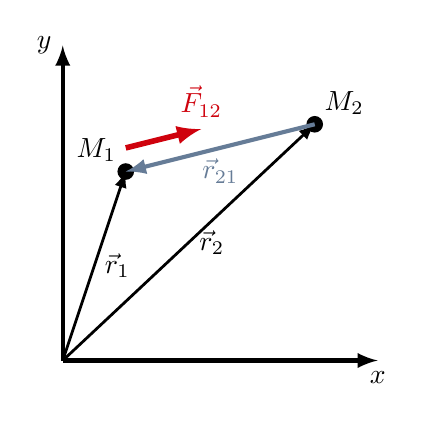
\begin{tikzpicture}
\tikzmath{
\L=4;
}
\scalebox{1}{

\coordinate (M1) at (0.2*\L, 0.6*\L);
\coordinate (M2) at (0.8*\L, 0.75*\L);

\draw[-latex,line width=1.5] (0,0) -- (\L,0) node[below]{$x$};
\draw[-latex,line width=1.5] (0,0) -- (0,\L) node[left]{$y$};

\fill (M1) circle (3pt) node[above left]{$M_1$};
\fill (M2) circle (3pt) node[above right]{$M_2$};

\draw[-latex,line width=1] (0,0) -- (M1) node[midway,right] {$\vec r_1$};
\draw[-latex,line width=1] (0,0) -- (M2) node[midway,right] {$\vec r_2$};

\draw[-latex,line width=2, color=myred] ($(M1)+(0,0.3)$) -- ($(M1)!0.4!(M2)+(0,0.3)$) node[above] {$\vec F_{12}$};
\draw[-latex,line width=1.5, color=myblue!60] (M2) -- (M1) node[midway,below] {$\vec r_{21}$};

}

\end{tikzpicture}
\captionof*{figure}{\textit{Vectors in Newton's Universal Theory of Gravity. The force on $M_1$ is in the opposite direction of $\vec r_{21}$.}}
\end{center}
}



%%%%%%%%%%%%%%%%%%%%%%%%%%%%%%%%
\subsection{Coulomb's Law}
\label{subsec:coulombslaw}
\twocolframesf{Coulomb's Law}
{
The force, $\vec F_{12}$, \textbf{on} charge $Q_1$ \textbf{from} charge $Q_2$ can be written as:
\begin{align*}
\vec F_{12} = k \frac{Q_1Q_2}{r_{21}^2}\hat r_{21}=k \frac{Q_1Q_2}{r_{21}^{\textcolor{myred}{3}}} \textcolor{myred}{\vec r_{21}}
\end{align*}
where:
\begin{itemize}
\item $\vec r_{21}=\vec r_2 - \vec r_1$ is the vector from $Q_2$ to $Q_1$.
\item $\hat r_{21}$ is the unit vector in the $\vec r_{21}$ direction.
\item $k=\SI{9.989e9}{Nm^2/C^2}$ is Coulomb's constant.
\item The force can be \textbf{attractive or repulsive}, depending on the product $Q_1Q_2$. If the charges are opposite, the product is negative and the force is attractive.
\end{itemize}

}
{
\begin{center}
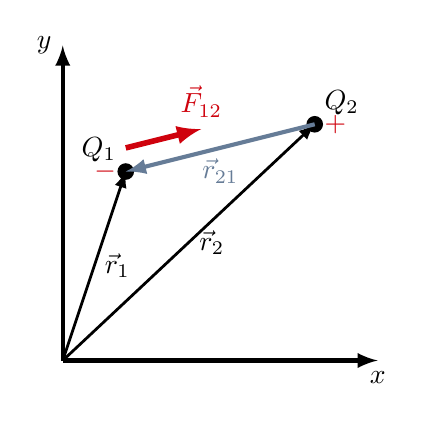
\begin{tikzpicture}
\tikzmath{
\L=4;
}
\scalebox{1}{

\coordinate (M1) at (0.2*\L, 0.6*\L);
\coordinate (M2) at (0.8*\L, 0.75*\L);

\draw[-latex,line width=1.5] (0,0) -- (\L,0) node[below]{$x$};
\draw[-latex,line width=1.5] (0,0) -- (0,\L) node[left]{$y$};

\fill (M1) circle (3pt) node[above left]{$Q_1$} node[left,color=myred]{$-$};
\fill (M2) circle (3pt) node[above right]{$Q_2$}node[right,color=myred]{$+$};

\draw[-latex,line width=1] (0,0) -- (M1) node[midway,right] {$\vec r_1$};
\draw[-latex,line width=1] (0,0) -- (M2) node[midway,right] {$\vec r_2$};

\draw[-latex,line width=2, color=myred] ($(M1)+(0,0.3)$) -- ($(M1)!0.4!(M2)+(0,0.3)$) node[above] {$\vec F_{12}$};
\draw[-latex,line width=1.5, color=myblue!60] (M2) -- (M1) node[midway,below] {$\vec r_{21}$};

}

\end{tikzpicture}
\captionof*{figure}{\textit{Vectors in Coulomb's Law. The force is attractive if the charges have opposite signs.}}
\end{center}
}


%%%%%%%%%%%%%%%%%%%%%%%%%%%%%%%%
\subsection{Gravity and the electric force}
\label{subsec:gravityandtheelectricforce}
\begin{frame}{Gravity and the Electric force}
\begin{itemize}
\item Mathematically, these are almost identical; instead of mass, we have electric charge (can think of gravitational mass as gravitational charge).
\item The main difference is that electric charges can be positive or negative, which can make the force attractive or repulsive.
\item Since we can define a gravitational field, $\vec g$ , we should be able to define an ``electric'' field, $\vec E$:
\begin{align*}
\vec F_g = m\vec g \quad\quad \vec F_E=q\vec E
\end{align*}
\item Since Gauss' Law can allow us to determine the gravitational field, it should also work for the electric field (next week's topic!).

\end{itemize}
\end{frame}


%%%%%%%%%%%%%%%%%%%%%%%%%%%%%%%%
\subsection{Inverse square laws and waves}
\label{subsec:inversesquarelawsandwaves}
\begin{frame}{Inverse square laws and waves}
Recall: to conserve energy, the intensity of a wave must decrease with the square of distance.
\begin{itemize}
\item So, maybe, the ``forces at a distance'' (gravity and Coulomb) are somehow transmitted by a wave?
\item Coulomb Force is actually transmitted by light waves!
\item Gravity is transmitted by waves (Nobel Prize 2017)!
\end{itemize}
\end{frame}


%%%%%%%%%%%%%%%%%%%%%%%%%%%%%%%%




%%%%%%%%%%%%%

\section{The Electric Field}
\label{sec:thelectricfield}
\title{The Electric Field}


%%%%%%%%%%%%%%%%%%%%%%%%%
\begin{frame}
\titlepage
\thispagestyle{empty}
\end{frame}


%%%%%%%%%%%%



%%%%%%%%%%%%%%%%%%%%%%%%%%%%%%%%
\subsection{Derivation}
\label{subsec:derivation}
\begin{frame}{The electric field}
\begin{itemize}
\item Consider the electric force from 2 stationary charges:
\begin{align*}
\vec F = \vec F_1 + \vec F_2=k\frac{qQ_1}{r_1^2}\hat r_1+k\frac{qQ_2}{r_2^2}\hat r_2
\end{align*}
\item Since $q$ is a scalar, it can be factored out:
\begin{align*}
\vec F =q\left( k\frac{Q_1}{r_1^2}\hat r_1+k\frac{Q_2}{r_2^2}\hat r_2\right)
\end{align*}
\item We can easily get the force vector for $q\to -2q$ by just multiplying the part in parenthesis by $-2q$ instead of $q$.
\item The part in parenthesis is Force per Charge, or Electric field:
\begin{align*}
\vec E = \frac{\vec F}{q}
\end{align*}
\end{itemize}

\end{frame}


%%%%%%%%%%%%%%%%%%%%%%%%%%%%%%%%
\begin{frame}{Recall, gravitational field outside a spherical mass}
\begin{itemize}
\item At some distance $r$ from a (spherical) object of mass $M$, a mass $m$ feels a force:
\begin{align*}
\vec F = -G\frac{mM}{r^2}\hat r
\end{align*}
\item Force per unit mass (gravitational field) outside of a spherical body:
\begin{align*}
\vec g = \frac{F}{m}=-G\frac{M}{r^2}
\end{align*}
\item At the surface of the Earth (of radius, $R$):
\begin{align*}
\vec g = \frac{F}{m}=-G\frac{M}{R^2}
\end{align*}
\end{itemize}

\end{frame}


%%%%%%%%%%%%%%%%%%%%%%%%%%%%%%%%
\begin{frame}{Electric field}
\begin{itemize}
\item If you have a point charge, $Q$ at the origin, you can calculate the electric field vector at any point in space, at a position $\vec r$ :
\begin{align*}
\vec E = k\frac{Q}{r^2}\hat r
\end{align*}
\item To find the force vector on some other charge, $q$, you just multiply the value of the electric field by $q$:
\begin{align*}
\vec F_q=q\vec E
\end{align*}
\item The electric field is a ``Vector Field'' (it is a function that you can evaluate anywhere in space to obtain a vector).
\end{itemize}
\end{frame}


%%%%%%%%%%%%%%%%%%%%%%%%%%%%%%%%
\subsection{Field lines}
\label{subsec:fieldlines}
\twocolframesf{Visualizing the electric field: Field Lines}
{
\begin{itemize}
\item We can draw ``field lines'' that tell us how to determine the electric field vector at some point in space:
\begin{itemize}
\item The more lines there are in an area of space, the stronger the electric field (the longer the vector) and corresponding force.
\item The electric field vector is always tangent to the field lines.
\item The electric field vector is always \textbf{in the direction of the force that a positive charge would feel}.
\end{itemize}
\end{itemize}
}
{
\vspace{-1.5cm}
\begin{center}
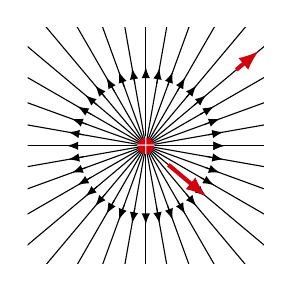
\begin{tikzpicture}
\tikzmath{
\L=2.5;
}
\scalebox{1}{

\begin{scope}
\clip (-0.6*\L,-0.6*\L) rectangle (0.6*\L,0.6*\L);
\foreach \th in {0,10,...,360}{
\draw (0,0) -- (\th:\L);
\draw[latex-] (\th:0.4*\L) -- +(\th:-0.2);
}
\end{scope}
\fill[color=myred] (0,0) circle (3pt);
\node[color=white] at (0,0){+};

\draw[latex-,line width=1.5,color=myred] (40:0.75*\L) -- +(40:-0.15*\L);
\draw[latex-,line width=1.5,color=myred] (-40:0.4*\L) -- +(-40:-0.25*\L);

}
\end{tikzpicture}
\captionof*{figure}{\textit{Electric field lines out of a positive point charge.}}
\end{center}


\begin{center}
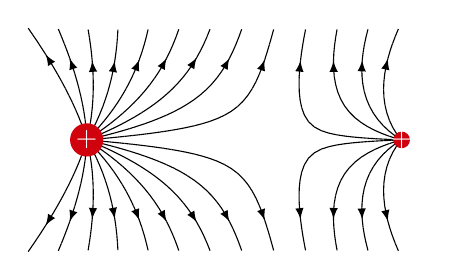
\begin{tikzpicture}
\tikzmath{
\xe=-2;%Coordinates of first mass/charge (Earth)
\ye=0;
\xm=2;%Coordinates of first mass/charge (Moon)
\ym=0;
\mee=1;% Mass/charge of first mass (Earth)
\mmm=0.6;% Mass/charge of first mass (Earth)
\dl=0.1;%scale factor to advance along the field line
\n=35;%number of points to find in the line (make as small as possible to reach the point you want!)
}

\scalebox{1}{
%Top field lines (xst is the starting x position of the field line)
\foreach \xst in {-2.8,-2.4,...,2.4}{
  \tikzmath{
  \yst=1.5; %all field lines start at yst
  \x=\xst;
  \y=\yst;
  %
  %generate points on the line (keeps finding the next point)
  int \i;
  %note that this also creates \mypairx and \mypairy!
  coordinate \mypair;
  for \i in {1,...,\n}{
    %First mass (earth)
    \re=(\x-\xe)*(\x-\xe)+(\y-\ye)*(\y-\ye)+0.0001;
    \Fex=\mee*(\x-\xe)/\re;
    \Fey=\mee*(\y-\ye)/\re;
    %Second mass (moon)
    \rm=(\x-\xm)*(\x-\xm)+(\y-\ym)*(\y-\ym)+0.0001;
    \Fmx=\mmm*(\x-\xm)/\rm;
    \Fmy=\mmm*(\y-\ym)/\rm;
    %Total force:
    \Fx=\Fex+\Fmx;
    \Fy=\Fey+\Fmy;
    \Fn=sqrt(\Fx*\Fx+\Fy*\Fy)+0.0001;
    \dx=\Fx/\Fn*\dl;
    \dy=\Fy/\Fn*\dl;
    \x=\x-\dx;
    \y=\y-\dy;
    \mypair{\i}=(\x,\y);
    };
  }
  %Draw that field line
  \foreach \i in {2,...,\n}{
    \tikzmath{
    int \im;
    \im=\i-1;
    }
    \draw (\mypair{\im}) -- (\mypair{\i});
    \ifthenelse{\im =5}{\draw[latex-] (\mypair{\im}) -- (\mypair{\i})}{};%draw arrow on the fifth point
  }

}%end of loop over x

%Bottom field lines
\foreach \xst in {-2.8,-2.4,...,2.4}{
  \tikzmath{
  \yst=-1.5;
  \x=\xst;
  \y=\yst;
  %
  %generate points on the line
  int \i;
  %note that this also creates \mypairx and \mypairy!
  coordinate \mypair;
  for \i in {1,...,\n}{
    %First mass (earth)
    \re=(\x-\xe)*(\x-\xe)+(\y-\ye)*(\y-\ye)+0.0001;
    \Fex=\mee*(\x-\xe)/\re;
    \Fey=\mee*(\y-\ye)/\re;
    %Second mass (moon)
    \rm=(\x-\xm)*(\x-\xm)+(\y-\ym)*(\y-\ym)+0.0001;
    \Fmx=\mmm*(\x-\xm)/\rm;
    \Fmy=\mmm*(\y-\ym)/\rm;
    %Total force:
    \Fx=\Fex+\Fmx;
    \Fy=\Fey+\Fmy;
    \Fn=sqrt(\Fx*\Fx+\Fy*\Fy)+0.0001;
    \dx=\Fx/\Fn*\dl;
    \dy=\Fy/\Fn*\dl;
    \x=\x-\dx;
    \y=\y-\dy;
    \mypair{\i}=(\x,\y);
    };
  }
  %Draw that field line
  \foreach \i in {2,...,\n}{
    \tikzmath{
    int \im;
    \im=\i-1;
    }
    \draw (\mypair{\im}) -- (\mypair{\i});
    \ifthenelse{\im =5}{\draw[latex-] (\mypair{\im}) -- (\mypair{\i})}{};
  }

}%end of loop over x

%Draw the charges
\fill[color=myred] ((\xe,\ye)  circle (6pt);
\node[color=white] at (\xe,\ye) {$+$};

\fill[color=myred] (\xm,\ym) circle (3pt);
\node[color=white] at (\xm,\ym){$+$};


}

\end{tikzpicture}
\captionof*{figure}{\textit{Electric field lines from two different positive charges.}}
\end{center}


}

%%%%%%%%%%%%%%%%%%%%%%%%%%%%%%%%



















%%%%%%%%%%%%%%%%%%%%%%%%%%%%%%%%


%%%%%%%%%%%%%%%%%%%%%%%%%%%%%%%%
\subsection{Superposition}
\label{subsec"superposition}
\twocolframesf{Electric field and superposition}
{
\begin{itemize}
\item If there are multiple charges, one can add the electric field from each charge to get the total electric field at one point in space.
\item If we have continuous charge distributions (as opposed to point charges), then we can model those distributions as being the sum of many individual point charges.
\item The total electric field can be found by adding the infinitesimal electric fields from each (point) charge element:
\begin{align*}
d\vec E &= k\frac{dq}{r^2}\hat r\\
\vec E &= \int d\vec E
\end{align*}
\end{itemize}
}
{
\begin{center}
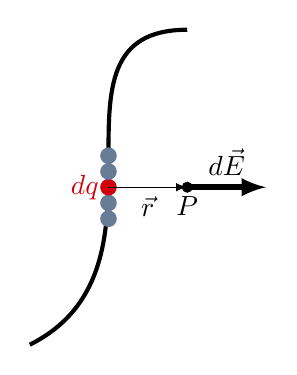
\begin{tikzpicture}

\scalebox{1}{

\draw[line width=1.5] (0,0) ..controls (2,1) and (0,4).. (2,4);


\fill[myblue!60] (1,1.6) circle(3pt);
\fill[myblue!60] (1,1.8) circle(3pt);
\fill[myred] (1,2) circle(3pt) node[left]{$dq$};
\fill[myblue!60] (1,2.2) circle(3pt);
\fill[myblue!60] (1,2.4) circle(3pt);

\fill (2,2) circle (2pt) node[below]{$P$};
\draw[-latex] (1,2) -- (2,2) node[midway,below]{$\vec r$};
\draw[-latex, line width=2] (2,2) -- +(1,0) node[midway,above]{$d\vec E$};
}
\end{tikzpicture}
\captionof*{figure}{\textit{To determine the electric field at point $P$ from a charge distribution, model the distribution as a collection of point charges, $dq$, and add those fields together.}}
\end{center}
}


%%%%%%%%%%%%%%%%%%%%%%%%%%%%%%%%



%%%%%%%%%%%%%%%%%%%%%%%%%%%%%%%%
\subsection{Electric field from a half-ring of charge}
\label{subsec:electricfieldfromahalfringofcharge}
\twocolframesf{Electric field from a half-ring of charge}
{
\only<1-6>{
\begin{enumerate}
\item Make a \textit{good} diagram.
\item<2-> Choose a charge element, \textcolor{myred}{$dq$}.
\item<3-> Draw the electric field element, \textcolor{myred}{$d\vec E$}, due to $dq$.
\item<4-> Write the electric field element, \textcolor{myred}{$d\vec E$}, using relevant variables:
\begin{align*}
d\vec E = \frac{k dq}{R^2}(\cos\theta \hat x -\sin\theta \hat y) = dE_x\hat x + dE_y \hat y
\end{align*}
\item<5-> Think of symmetry! ($\int dE_y=0$)
\item<6-> Write the electric field as the sum of the $d\vec E$:
\begin{align*}
\vec E = \int d\vec E = \left(\int dE_x\right)\hat x + \cancelto{0}{\left(\int dE_y\right)}\hat y
\end{align*}
\end{enumerate}
}
\only<7->{
\begin{enumerate}
\setcounter{enumi}{6}
\item We will choose, $\theta$, as the the integration variable:
\begin{align*}
E_x = \int dE_x =  \int_{\frac{-\pi}{2}}^{\frac{\pi}{2}} \frac{k dq}{R^2}\cos\theta
\end{align*}
\item Introduce charge per unit length, $\lambda=\frac{Q}{\pi R}$:
\begin{align*}
dq &= \lambda R d\theta=\frac{Q}{\pi R} Rd\theta=\frac{Q}{\pi}d\theta\\
\therefore E_x &= \int_{\frac{-\pi}{2}}^{\frac{\pi}{2}} \frac{k Q }{\pi R^2}\cos\theta d\theta\\
&=\frac{k Q }{\pi R^2} \int_{\frac{-\pi}{2}}^{\frac{\pi}{2}} \cos\theta d\theta = \frac{k Q }{\pi R^2}\left[\sin\theta\right]_{\frac{-\pi}{2}}^{\frac{\pi}{2}} =  \frac{2k Q }{\pi R^2}
\end{align*}
\end{enumerate}
}
}
{
\begin{center}
\begin{tikzpicture}
\tikzmath{
\R=2;
}
\scalebox{1}{

\draw[line width=3] (0,\R) arc(90:270:\R);
\draw[-latex] (0,0) -- +(1,0) node[below]{$x$};
\draw[-latex] (0,0) -- +(0,1) node[left]{$y$};
\node[above] at (110:\R) {$Q$};

\only<2->{
\draw[line width=3, color=myred] (130:\R) arc (130:140:\R) node[midway,above]{$dq$};
\draw[dashed, line width =1.5, color=myred] (0,0) -- (180:\R);
\draw[dashed, line width =1.5, color=myred] (0,0) -- (135:\R) node[midway,above]{$R$};
\draw[color=myred] (180:0.7) arc(180:135:0.7) node[midway,left]{$\theta$};
}

\only<3->{
\draw[-latex, line width=2, color=myred] (0,0) -- (-45:0.5*\R) node[below]{$d\vec E$};
}

\only<5>{
\draw[line width=3, color=myblue!60] (220:\R) arc (220:230:\R) node[midway,below]{$dq'$};
\draw[-latex, line width=2, color=myblue!60, dashed] (0,0) -- (45:0.5*\R) node[above]{$d \pvec E'$};
\draw[dashed, line width =1.5, color=myblue!60] (0,0) -- (225:\R);
}


}
\end{tikzpicture}
\captionof*{figure}{\textit{Modeling the electric field from a half-ring of charge, $Q$.}}
\end{center}
}



%%%%%%%%%%%%%%%%%%%%%%%%%%%%%%%%
\subsection{Electric field from an infinite line charge}
\label{subsec:electricfieldfromaninfinitelinecharge}
\twocolframesf{Electric field from an infinite line charge}
{
\only<1-5>{
\begin{enumerate}
\item Make a \textit{good} diagram.
\item<2-> Choose a charge element, \textcolor{myred}{$dq$}.
\item<3-> Draw the electric field element, \textcolor{myred}{$d\vec E$}, due to $dq$.
\item<4-> Write the electric field element, \textcolor{myred}{$d\vec E$}, using relevant variables:
\begin{align*}
d\vec E = \frac{k dq}{r^2}(\cos\theta \hat x -\sin\theta \hat y) = dE_x\hat x + dE_y \hat y
\end{align*}
\item<5-> Think of symmetry! ($\int dE_y=0$):
\begin{align*}
\vec E = \left(\int \frac{k dq}{r^2}\cos\theta\right) \hat x
\end{align*}
%\item<6-> Write the electric field as the sum of the $d\vec E$:
%\begin{align*}
%\vec E = \int d\vec E = \left(\int dE_x\right)\hat x + \cancelto{0}{\left(\int dE_y\right)}\hat y
%\end{align*}
\end{enumerate}
}
\only<6-7>{
\vspace{-0.75cm}
\begin{align*}
\vec E = \left(\int \frac{k dq}{r^2}\cos\theta\right) \hat x
\end{align*}
\vspace{-0.5cm}
\begin{enumerate}
\setcounter{enumi}{5}
\item<6-> We can integrate over $\theta$ or $y$, we choose $y$. Anything that changes with different $dq$ needs to be expressed with $y$ and constants:
\begin{align*}
dq = \lambda dy\;\;\text{and}\;\;  r^2=R^2+y^2 \;\;\text{and}\;\; \cos\theta=\frac{R}{\sqrt{R^2+y^2}}
\end{align*}
\item<7-> All together:
\begin{align*}
E_x = \int_{-\infty}^{+\infty} \frac{k \lambda dy R}{\left(y^2+R^2  \right)^{\frac{3}{2}}}=k\lambda R\int_{-\infty}^{+\infty} \frac{ dy}{\left(y^2+R^2  \right)^{\frac{3}{2}}}
\end{align*}
ask your math friend for help, look it up...
\end{enumerate}
}
\only<8->{
\vspace{-0.75cm}
\begin{align*}
\vec E = \left(\int \frac{k dq}{r^2}\cos\theta\right) \hat x
\end{align*}
\vspace{-0.5cm}
\begin{itemize}
\item<8-> What if we integrate over $\theta$?
\only<9->{
\vspace{-0.5cm}
\begin{align*}
y=R\tan\theta \;\;\rightarrow\;\;\frac{dy}{d\theta}=\frac{R}{\cos^2\theta}\\
\therefore dq = \lambda dy=\lambda\frac{R}{\cos^2\theta} d\theta \;\;\text{and}\;\;  r^2=\frac{R^2}{\cos^2\theta}
\end{align*}}
\item<10-> All together:
\begin{align*}
E_x &= \int_{-\frac{\pi}{2}}^{+\frac{\pi}{2}} k\lambda\frac{Rd\theta}{\cos^2\theta}\frac{\cos^2\theta}{R^2}\cos\theta=\frac{k\lambda}{ R}\int_{-\frac{\pi}{2}}^{+\frac{\pi}{2}} \cos\theta d\theta\\
 &= \frac{2k\lambda}{ R}
\end{align*}
\end{itemize}
}
}
{
\begin{center}
\begin{tikzpicture}
\tikzmath{
\L=5;
\R=2;
\thq=30;
\hq=\R*tan(\thq);
\dx=0.4;
}
\scalebox{1}{

\draw[line width=3] (-\R,-\L/2) -- (-\R,\L/2);
\draw[-latex] (0,0) -- +(1,0) node[below]{$x$};
\draw[-latex] (0,0) -- +(0,1) node[left]{$y$};
\fill (0,0) circle (2pt);
\draw[latex-latex, line width=1.5] (0,0) -- (-\R, 0) node[midway,below]{$R$};
\node[right] at (-\R,\L/2) {$\lambda$};

\only<2->{
\draw[line width=3, color=myred] (-\R,\hq-0.5*\dx) -- +(0,\dx) node[midway,left]{$dq$};
\node[right, color=myred] at (-\R,0.5*\hq){$y$};
\draw[dashed, line width =1.5, color=myred] (0,0) -- (-\R,\hq) node[midway,above]{$r$};
\draw[color=myred] (180:0.7) arc(180:180-\thq:0.7) node[midway,left]{$\theta$};
}

\only<3->{
\draw[-latex, line width=2, color=myred] (0,0) -- (-\thq:1) node[below]{$d\vec E$};
}

\only<5>{
\draw[line width=3, color=myblue!60] (-\R,-\hq-0.5*\dx) -- +(0,-\dx) node[midway,left]{$dq'$};
\draw[-latex, line width=2, color=myblue!60, dashed] (0,0) -- (\thq:1) node[above]{$d \pvec E'$};
\draw[dashed, line width =1.5, color=myblue!60] (0,0) -- (-\R,-\hq) ;
}


}
\end{tikzpicture}
\captionof*{figure}{\textit{Modeling the electric field at a distance, $R$, from an infinite line of charge.}}
\end{center}
}


%%%%%%%%%%%%%%%%%%%%%%%%%%%%%%%%


%%%%%%%%%%%%%%%%%%%%%%%%%%%%%%%%
\subsection{2D infinite plane}
\label{subsec:2dinfiniteplane}
\twocolframesf{2D infinite plane}
{
\begin{itemize}
\item If you have a continuous 2D (3D) charge distribution, model it as the sum of electric fields from 1D (2D) charge distributions.
\item For example, for an infinite plane (2D), consider it has being made of many infinite lines of charge (1D), for which you just calculated the electric field.
\begin{itemize}
\item The plane has surface charge density, $\sigma$.
\item An infinite line of charge with width dy thus has linear charge density:
\begin{align*}
\lambda = \sigma dy
\end{align*}
\item Sum all of the electric fields from lines of charge at different values of $y$.
\end{itemize}

\end{itemize}
}
{
\vspace{-1cm}
\begin{center}
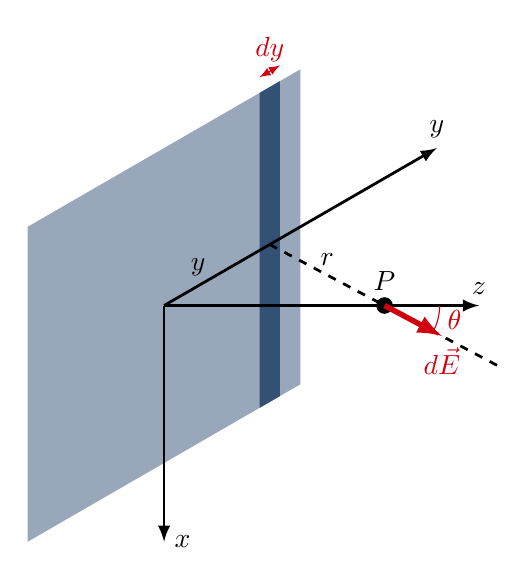
\begin{tikzpicture}
\tikzmath{
\L=4;
\thyz=30;%perspective angle
\Ly=4;
\dy=0.3;
}
\scalebox{1}{
\coordinate (P1) at ($(180+\thyz:\Ly/2)-(0,0.5*\L)$);
\coordinate (P2) at ($(P1)+(0,\L)$);
\coordinate (P3) at ($(P2)+(\thyz:\Ly)$);
\coordinate (P4) at ($(P3)+(0,-\L)$);
%strip
\coordinate (P5) at ($(\thyz:0.35*\Ly)-(0,0.5*\L)$);
\coordinate (P6) at ($(P5)+(0,\L)$);
\coordinate (P7) at ($(P6)+(\thyz:\dy)$);
\coordinate (P8) at ($(P7)+(0,-\L)$);

\fill[color=myblue!40] (P1) -- (P2) -- (P3) -- (P4) -- cycle;
\fill[color=myblue!80] (P5) -- (P6) -- (P7) -- (P8) -- cycle;
\draw[line width=1,-latex] (0,0) -- +(\thyz:\Ly) node[above]{$y$};
\draw[line width=1,-latex] (0,0) -- +(\Ly,0) node[above]{$z$};
\draw[line width=1,-latex] (0,0) -- +(0,-0.75*\L) node[right]{$x$};

\coordinate (PY) at (\thyz:0.35*\Ly+0.5*\dy);
\coordinate (PZ) at (0.7*\Ly,0);
\coordinate (PE) at ($(PY)!1.5!(PZ)$);

\node[above] at (\thyz:\Ly/8) {$y$};
\fill (PZ) circle (3pt) node[above=2pt]{$P$};
\draw[line width = 1, dashed ] (PY) -- ($(PY)!2!(PZ)$);
\node[above] at ($(PY)!0.5!(PZ)$) {$r$};
\draw[line width = 2, color=myred, -latex] (PZ) -- (PE) node[below]{$d\vec E$};
\draw[color=myred] ($(PZ)+(0.7,0)$) arc(0:-30:0.7)node[midway,right]{$\theta$};
\draw[latex-latex,color=myred] ($(P6)+(0,0.2)$) -- ($(P7)+(0,0.2)$) node[midway,above]{$dy$};
}
\end{tikzpicture}
\captionof*{figure}{\textit{The electric field from an infinite plane with charge per unit area, $\sigma$. By symmetry, the net field will be in the $y$ direction.}}
\end{center}
}


%%%%%%%%%%%%%%%%%%%%%%%%%%%%%%%%
\subsection{2D infinite plane, method 2}
\label{subsec:2dinfiniteplanemethod2}
\twocolframesf{{2D infinite plane, different method}}
{
\begin{itemize}
\item You can model the infinite plane as the sum of rings. 
\item A ring of width $dr$ has  total charge given by:
\begin{align*}
dq=\sigma 2 \pi r dr
\end{align*}
\item Sum all of the electric fields from all of the rings, from $r=0$ to $r=\infty$.
\end{itemize}
}
{
\begin{center}
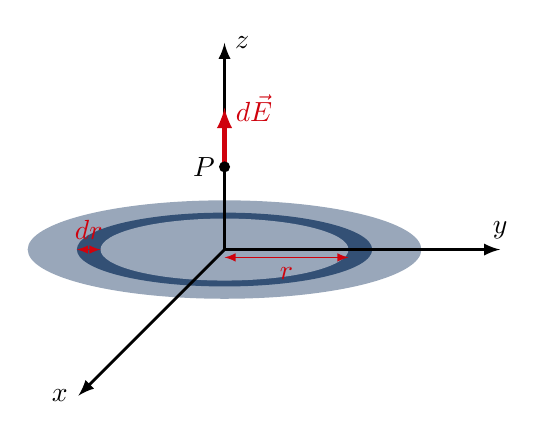
\begin{tikzpicture}
\tikzmath{
\L=4;
\thyz=45;%perspective angle
\Ly=3.5;
\R=2.5;
\r=0.75*\R;
\dr=0.3;
}
\scalebox{1}{

\fill[color=myblue!40] (0,0) circle({\R} and {\R/4});
\fill[color=myblue!80] (0,0) circle({\r} and {\r/4});
\fill[color=myblue!40] (0,0) circle({\r-\dr} and {(\r-\dr)/4});

\draw[line width=1,-latex] (0,0) -- +(270-\thyz:0.75*\Ly) node[left]{$x$};
\draw[line width=1,-latex] (0,0) -- +(\Ly,0) node[above]{$y$};
\draw[line width=1,-latex] (0,0) -- +(0,0.75*\Ly) node[right]{$z$};

\draw[latex-latex,color=myred] (0,-0.1) -- +(\r-\dr,0) node[midway,below]{$r$};
\draw[latex-latex,color=myred] (-\r,0) -- +(\dr,0) node[midway,above]{$dr$};
\draw[-latex,color=myred, line width=1.5] (0,0.3*\Ly) -- +(0,0.75) node[right]{$d\vec E$};
\fill (0,0.3*\Ly) circle(2pt) node[left]{$P$};
}
\end{tikzpicture}
\captionof*{figure}{\textit{The electric field from an infinite plane with charge per unit area, $\sigma$. By symmetry, the net field will be in the $y$ direction.}}
\end{center}
}

%%%%%%%%%%%%%%%%%%%%%%%%%%%%%%%%



\subsection{Electric dipoles}
\label{subsec:electricdiapoles}
\twocolframesf{Electric dipoles}
{
\begin{itemize}
\item Dipoles are a pair of equal magnitude but opposite sign charges, $Q$, separated by a fixed distance, $l$.
\item For example, a water molecule can be modeled as a dipole.
\end{itemize}
}
{
\begin{center}
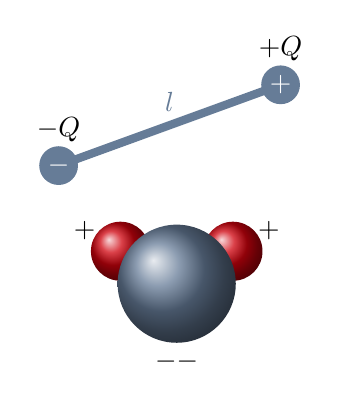
\begin{tikzpicture}
\tikzmath{
\L=3;
\R=0.75;
}
\scalebox{1}{
\draw[line width=3, color=myblue!60](0,0) -- (20:\L) node[midway,above]{$l$};
\fill[color=myblue!60] (0,0) circle (7pt) node[color=white]{$-$} node[above=5pt,color=black]{$-Q$};
\fill[color=myblue!60] (20:\L) circle (7pt) node[color=white]{$+$} node[above=5pt,color=black]{$+Q$};

\begin{scope}[shift={(0.5*\L,-0.5*\L)}]

\shade[ball color=myred] (30:1.1*\R) circle(0.5*\R);
\shade[ball color=myred] (150:1.1*\R) circle(0.5*\R);
\shade[ball color=myblue!60] (0,0) circle(\R);
\node[below] at (0,-\R){$--$};
\node at (30:1.8*\R){$+$};
\node at (150:1.8*\R){$+$};
\end{scope}

}
\end{tikzpicture}
\captionof*{figure}{\textit{A dipole and a water molecule.}}
\end{center}
}


%%%%%%%%%%%%%%%%%%%%%%%%%%%%%%%


%%%%%%%%%%%%%%%%%%%%%%%%%%%%%%%%
\twocolframesf{The dipole moment vector, $\vec p$}
{
\begin{itemize}
  \item We introduce the \textbf{dipole vector}, $\vec p$:
  \begin{itemize}
    \item Magnitude: $p=Ql$
    \item Direction from $-Q$ to $+Q$
  \end{itemize} 
  \item The net torque on the dipole is then given by:
  \begin{align*}
  \vec \tau &=\vec p \times \vec E\\
  \tau &= pE\sin\theta
  \end{align*}
\end{itemize} 
Check:
\begin{align*}
F_{\perp}&=QE\sin\theta\\
\therefore \tau &=F_\perp\frac{l}{2}+ F_\perp\frac{l}{2}\\
&= QEl\sin\theta=pE\sin\theta
\end{align*}
}
{
%\capfig{0.4}{figures/dipolefield}{A dipole in a field.}
\begin{center}
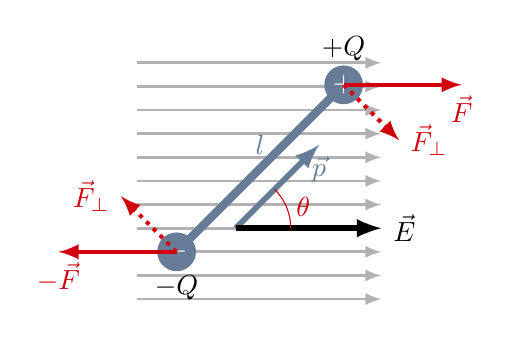
\begin{tikzpicture}
\tikzmath{
\L=3;
\R=0.75;
\th=45;
}
\scalebox{1}{

\foreach \h in {-0.6,-0.3,...,2.7}{
  \draw[color=black!30, line width=1,-latex] (-0.5,\h) -- (2.6,\h);
}
%\node[below] at (2.6,-0.6){$\vec E$};

\draw[line width=3, color=myblue!60](0,0) -- (\th:\L) node[midway,above]{$l$};
\fill[color=myblue!60] (0,0) circle (7pt) node[color=white]{$-$} node[below=5pt,color=black]{$-Q$};
\fill[color=myblue!60] (\th:\L) circle (7pt) node[color=white]{$+$} node[above=5pt,color=black]{$+Q$};
\draw[-latex,line width=2,color=myblue!60] ($ (0.75,0.3) $) -- +(\th:0.5*\L) node[below]{$\vec p$};
\draw[-latex,line width=2] ($ (0.75,0.3) $) -- (2.6,0.3) node[right]{$\vec E$};
\draw[color=myred]($ (0.75,0.3) +(0.7,0)$) arc(0:\th:0.7) node[midway,right]{$\theta$};

\draw[-latex,color=myred, line width=1.5] (0,0) -- (180:1.5) node[below]{$-\vec F$};
\draw[-latex,dotted,color=myred, line width=1.5] (0,0) -- (135:1) node[left]{$\vec F_\perp$};

\draw[-latex,color=myred, line width=1.5] (\th:\L) -- +(0:1.5) node[below]{$\vec F$};
\draw[-latex,dotted,color=myred, line width=1.5] (\th:\L) -- +(-45:1) node[right]{$\vec F_\perp$};
}
\end{tikzpicture}
\captionof*{figure}{\textit{A dipole, formed by two charges of magnitude, $Q$, a distance, $l$, apart in an electric field, $\vec E$.}}
\end{center}
}


%%%%%%%%%%%%%%%%%%%%%%%%%%%%%%%%




%%%%%%%%%%%%%%%%%%%%%%%%%%%%%%%%
\twocolframe{Dipole potential energy}
{
\begin{itemize}
  \item The potential energy is minimum when the dipole vector is parallel to the electric field.
  \item The potential energy is maximum when the dipole vector is anti-parallel to the electric field.
  \item We can write the potential energy:
  \begin{align*}
  U=-\vec p \cdot \vec E = -pE\cos\theta
  \end{align*}
\end{itemize} 
}
{
\begin{center}
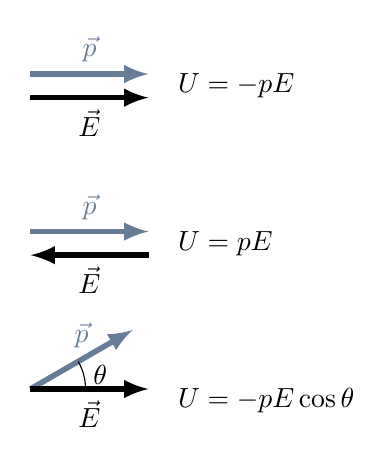
\begin{tikzpicture}
\tikzmath{
\th=30;
}
\scalebox{1}{

\draw[-latex,line width=2,color=myblue!60] (0,0) -- +(1.5,0) node[midway,above]{$\vec p$};
\draw[-latex,line width=2] (0,-0.3) -- +(1.5,0) node[midway,below]{$\vec E$};
\node[right] at (1.75,-0.15) {$U=-pE$};

\begin{scope}[shift={(0,-2)}]
\draw[-latex,line width=2,color=myblue!60] (0,0) -- +(1.5,0) node[midway,above]{$\vec p$};
\draw[latex-,line width=2] (0,-0.3) -- +(1.5,0) node[midway,below]{$\vec E$};
\node[right] at (1.75,-0.15) {$U=pE$};
\end{scope}

\begin{scope}[shift={(0,-4)}]
\draw[-latex,line width=2,color=myblue!60] (0,0) -- +(\th:1.5) node[midway,above]{$\vec p$};
\draw[-latex,line width=2] (0,0) -- +(1.5,0) node[midway,below]{$\vec E$};
\draw (0.7,0) arc(0:\th:0.7) node[midway,right]{$\theta$};
\node[right] at (1.75,-0.15) {$U=-pE\cos\theta$};
\end{scope}

}
\end{tikzpicture}
\captionof*{figure}{\textit{A dipole in an electric field.}}
\end{center}
}



%%%%%%%%%%%%%%%%%%%%%%%%%%%%%%%%



%%%%%%%%%%%%%%%%%%%%%%%%%%%%%%%%



%%%%%%%%%%%%%%%%%%%%%%%%%%%%%%%%



%%%%%%%%%%%%%%%%%%%%%%%%%%%%%%%%



%%%%%%%%%%%%%%%%%%%%%%%%%%%%%%%%



%%%%%%%%%%%%%%%%%%%%%%%%%%%%%%%%



%%%%%%%%%%%%%%%%%%%%%%%%%%%%%%%%



%%%%%%%%%%%%%%%%%%%%%%%%%%%%%%%%



%%%%%%%%%%%%%%%%%%%%%%%%%%%%%%%%



%%%%%%%%%%%%%%%%%%%%%%%%%%%%%%%%



%%%%%%%%%%%%%%%%%%%%%%%%%%%%%%%%



%%%%%%%%%%%%%%%%%%%%%%%%%%%%%%%%






\end{document}


